\documentclass[xcolor=dvipsnames]{beamer}
\usepackage[francais,american]{babel}
\usepackage[utf8x]{inputenc}
\usepackage{epstopdf}
\usepackage{pgf}
\usepackage{lmodern}

% Un thème standard
\setbeamercovered{transparent}
  \usetheme{Pittsburgh}
\beamertemplatenavigationsymbolsempty
\usepackage{colortbl} 
\usepackage{multirow}
\definecolor{kugreen}{RGB}{4,99,128}
\definecolor{kured}{RGB}{163,37,0}
\definecolor{kublue}{RGB}{70,109,220}

\definecolor{rt}{RGB}{225,225,225}
\definecolor{rt2}{RGB}{245,245,245}

\definecolor{purple2}{RGB}{178,20,4}
\definecolor{blue2}{RGB}{13,87,178}
\definecolor{purple3}{RGB}{115,178,29}
\definecolor{blue3}{RGB}{149,12,178}


\usecolortheme[named=kugreen]{structure}
\setbeamercolor{block body}{bg=rt2} 

\setbeamercolor{block title}{bg=rt} 
\usefonttheme[onlylarge]{structurebold}
\setbeamerfont*{frametitle}{size=\large,series=\bf}
\setbeamertemplate{navigation symbols}{}
\setbeamertemplate{footline}[frame number]
\setbeamertemplate{blocks}[rounded][shadow=false]


\setbeamercolor{section in head/foot}{use=structure,bg=structure.fg!10!bg}

\graphicspath{{./}}

\setbeamertemplate{footline}[default]

\begin{document}

\frame{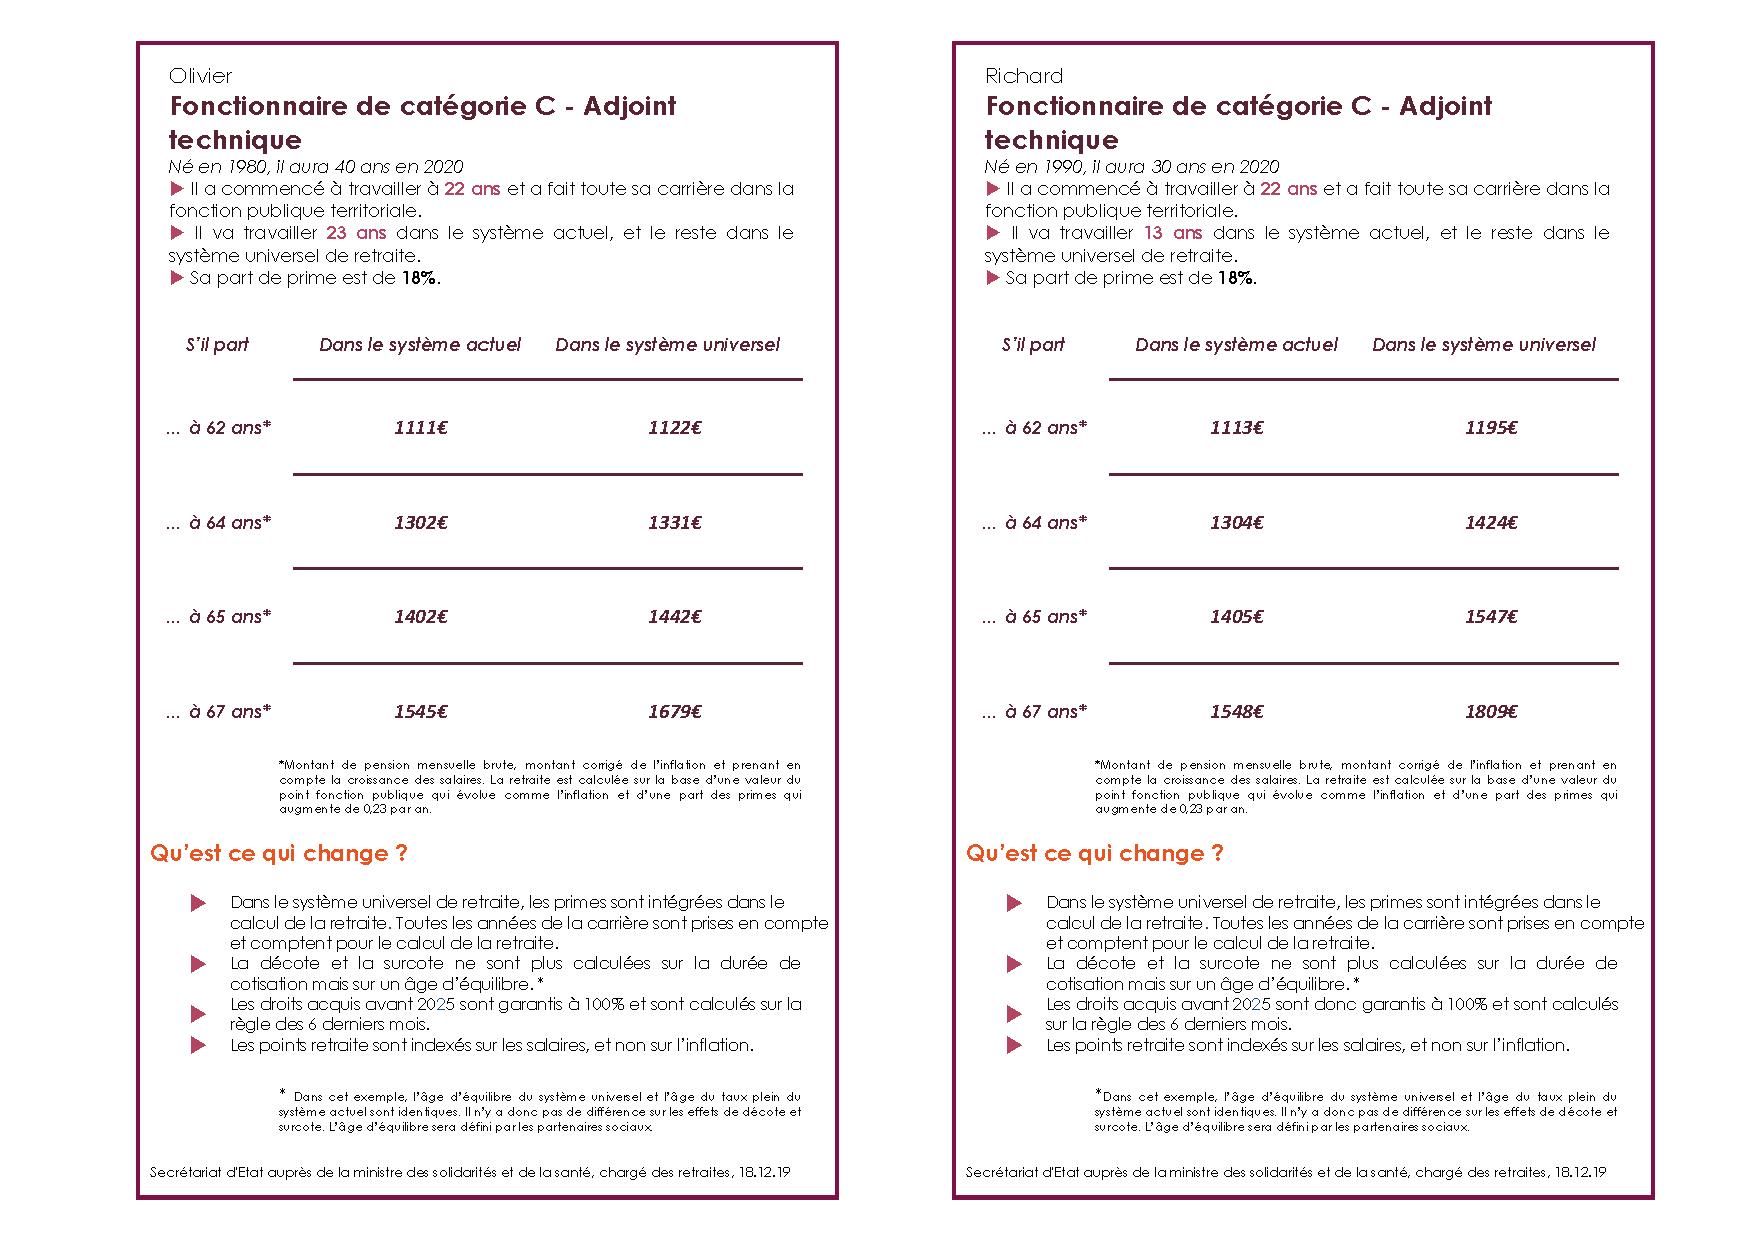
\includegraphics[width=\textwidth]{public2}}

\frame{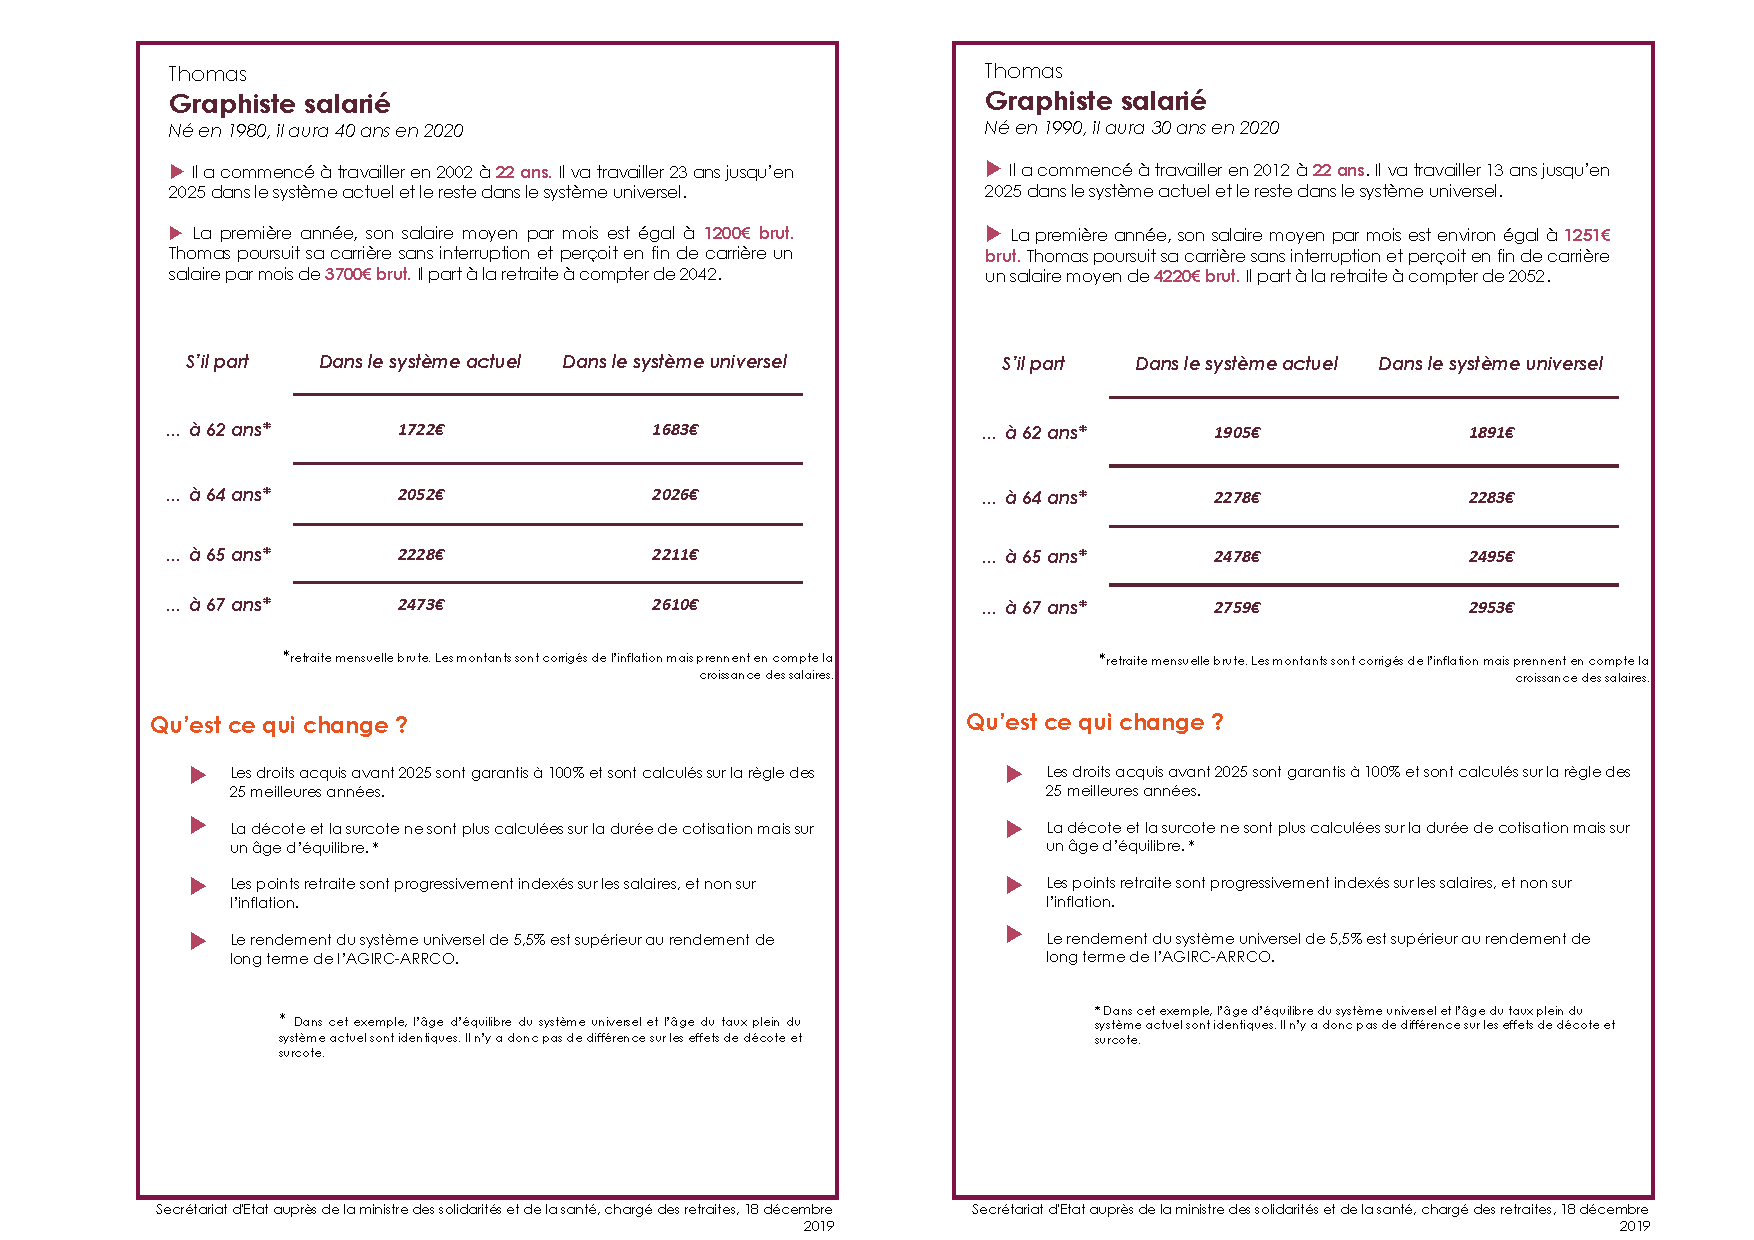
\includegraphics[width=\textwidth]{prive2}}

\frame{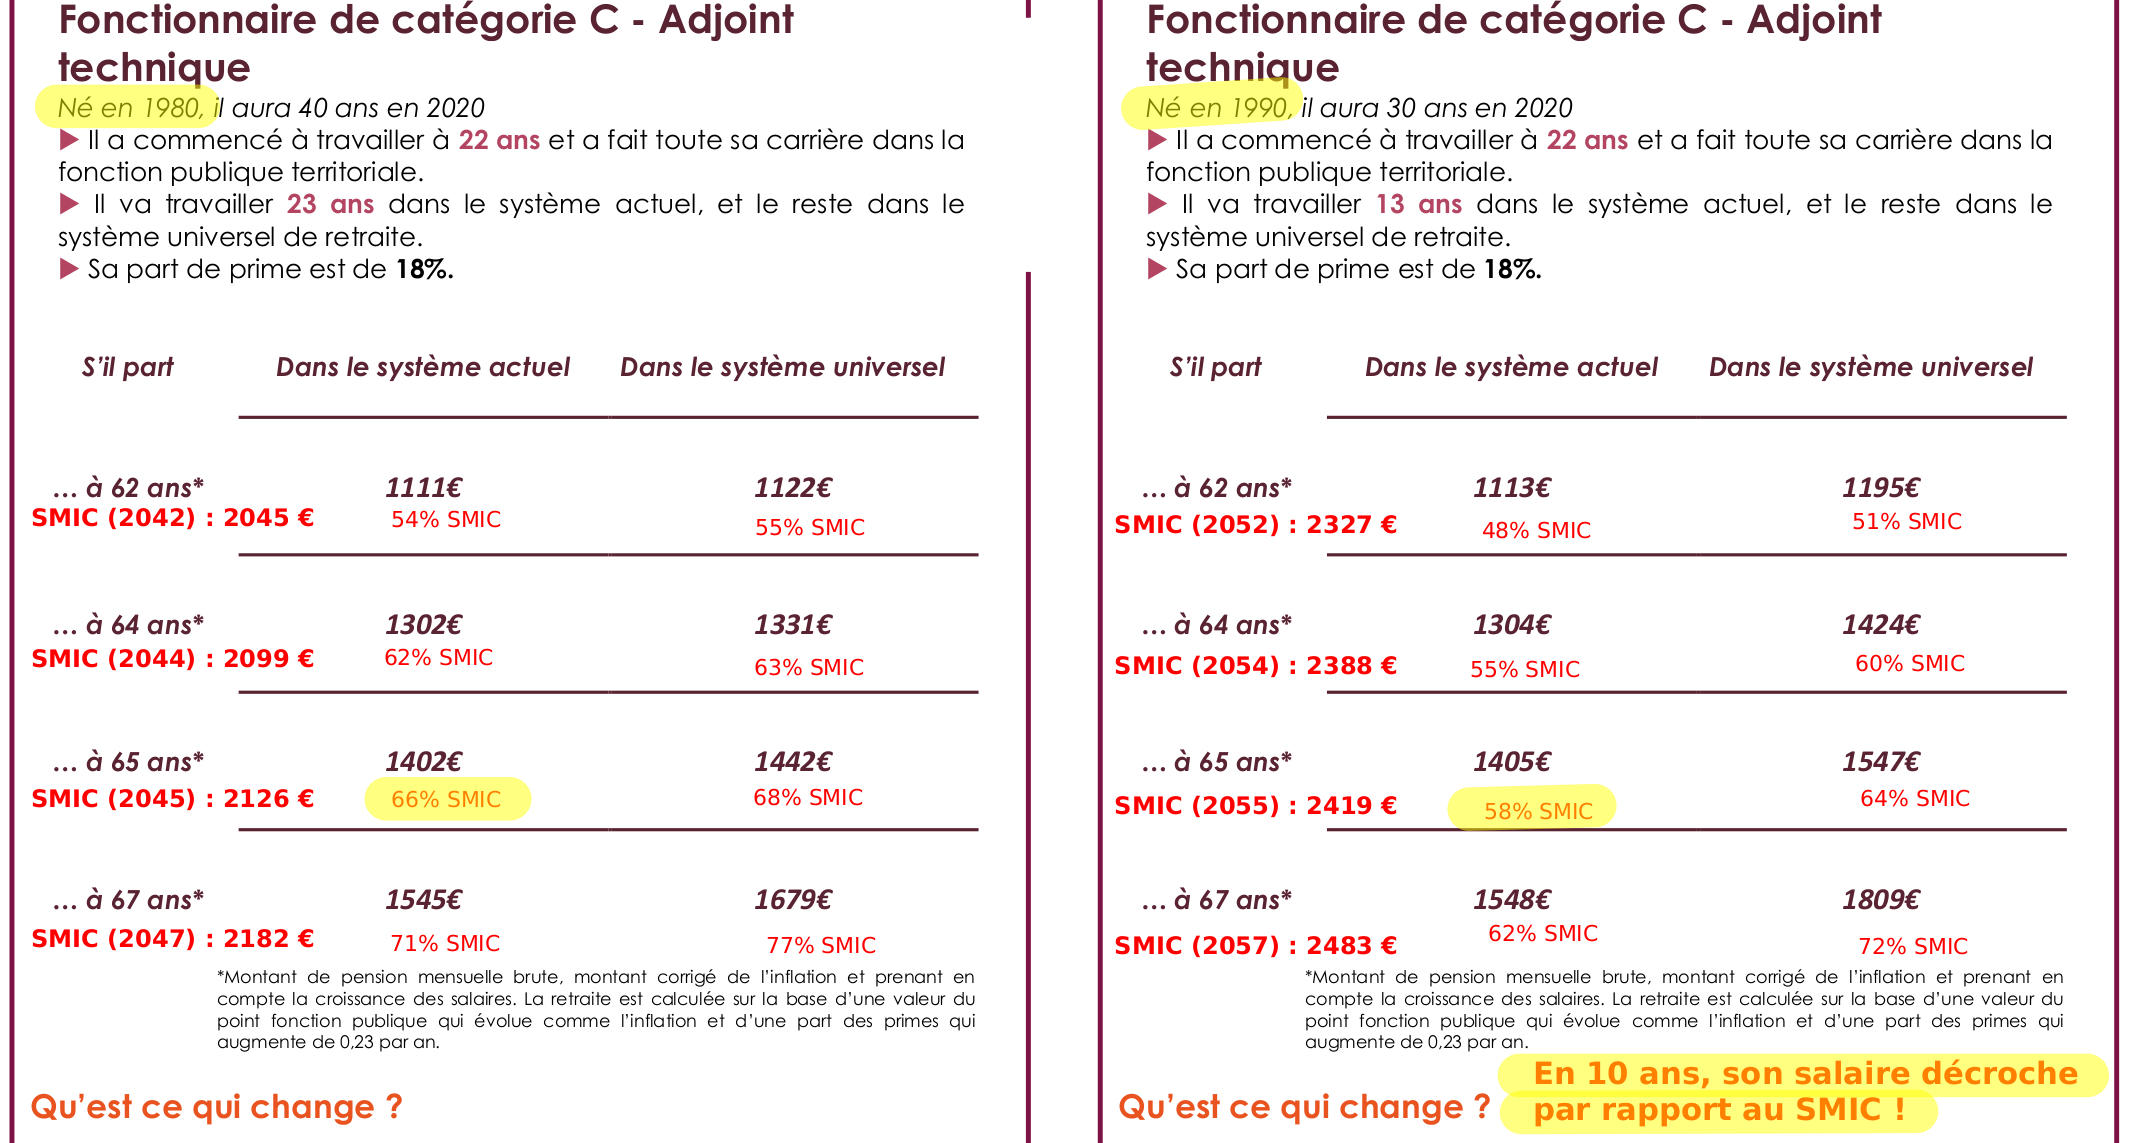
\includegraphics[width=\textwidth]{11}}

\frame{Personnel BIATSS commençant sa carrière à 22 ans en 2000:\\
  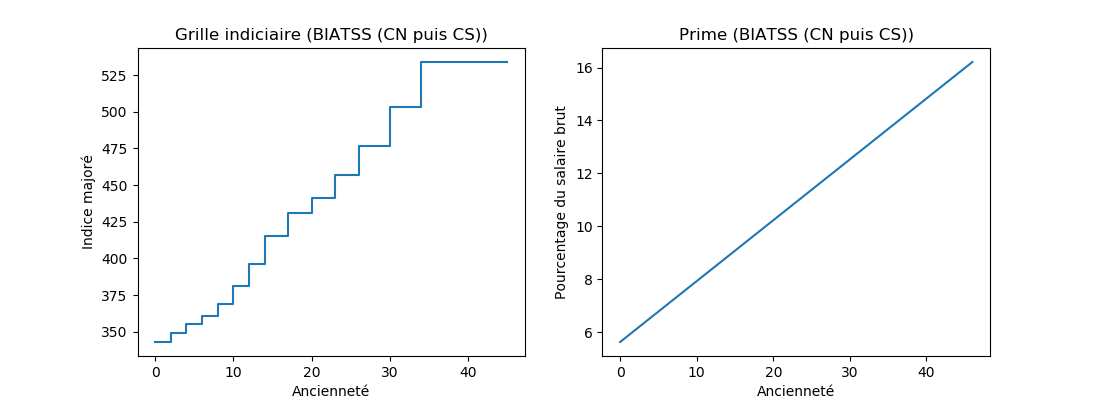
\includegraphics[width=\textwidth]{grille}\\
42 annuités en 2042, à 64 ans}

\frame{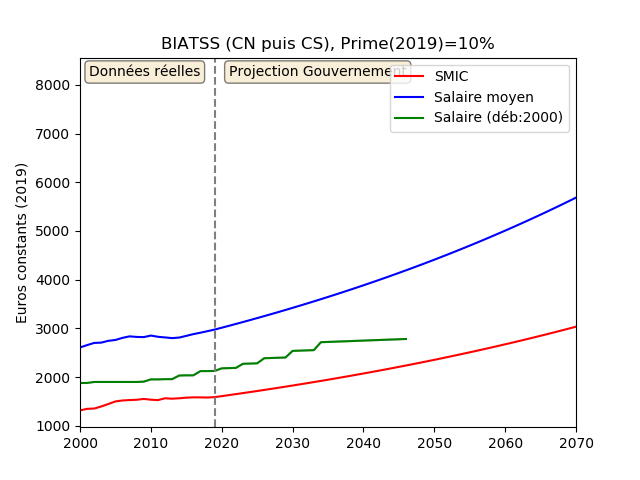
\includegraphics[width=\textwidth]{salaireEC}}

\frame{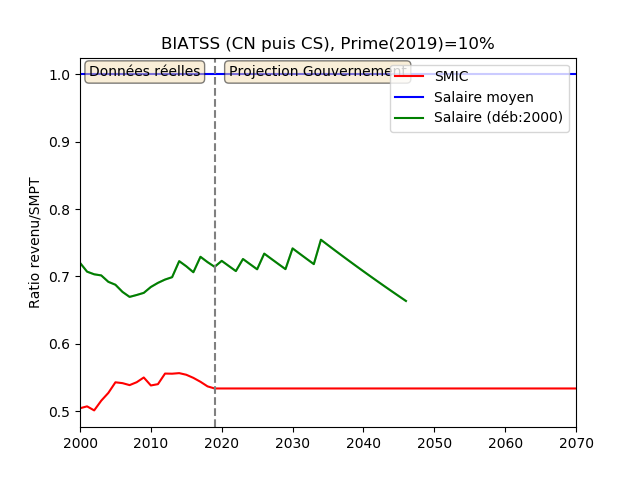
\includegraphics[width=\textwidth]{salaireRel}}



\frame{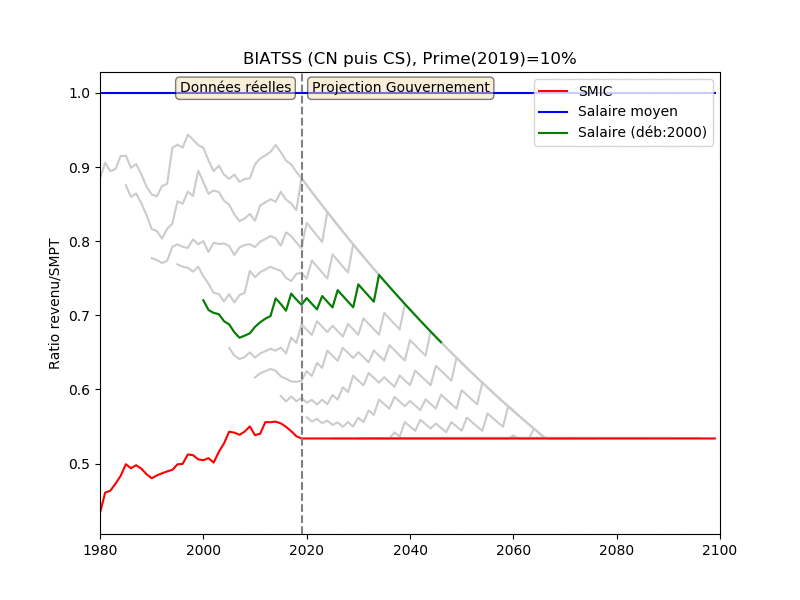
\includegraphics[width=\textwidth]{selonannee-4}}
\frame{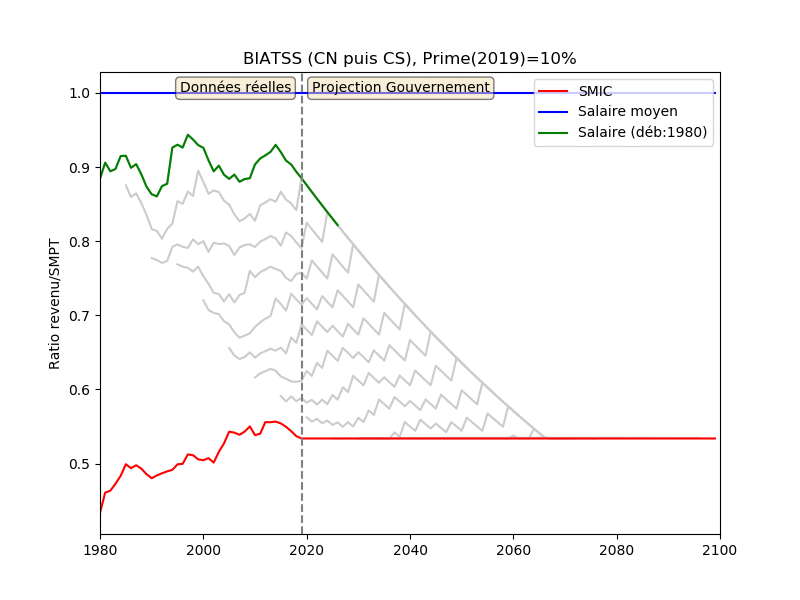
\includegraphics[width=\textwidth]{selonannee-0}}
\frame{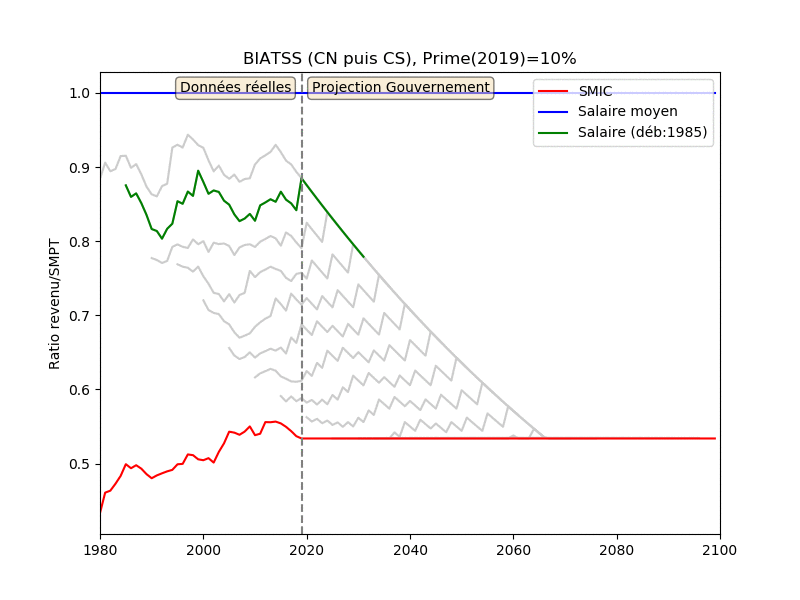
\includegraphics[width=\textwidth]{selonannee-1}}
\frame{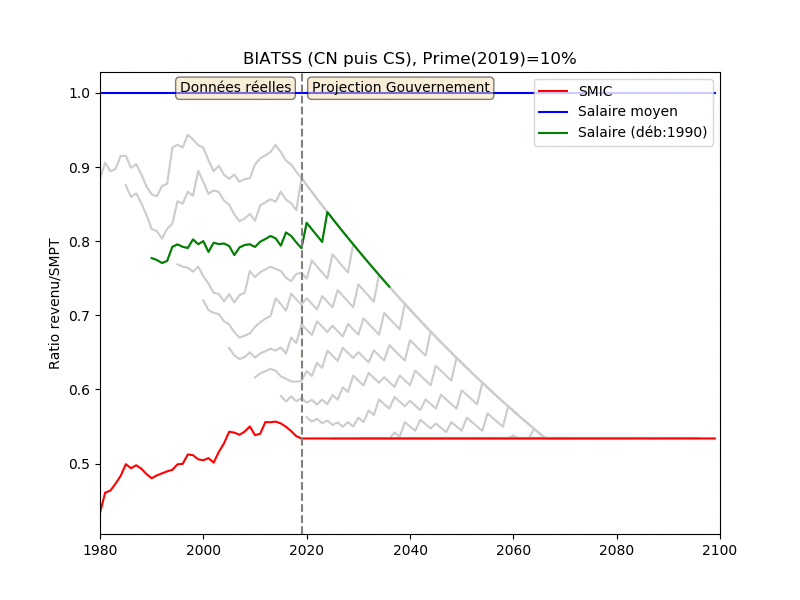
\includegraphics[width=\textwidth]{selonannee-2}}
\frame{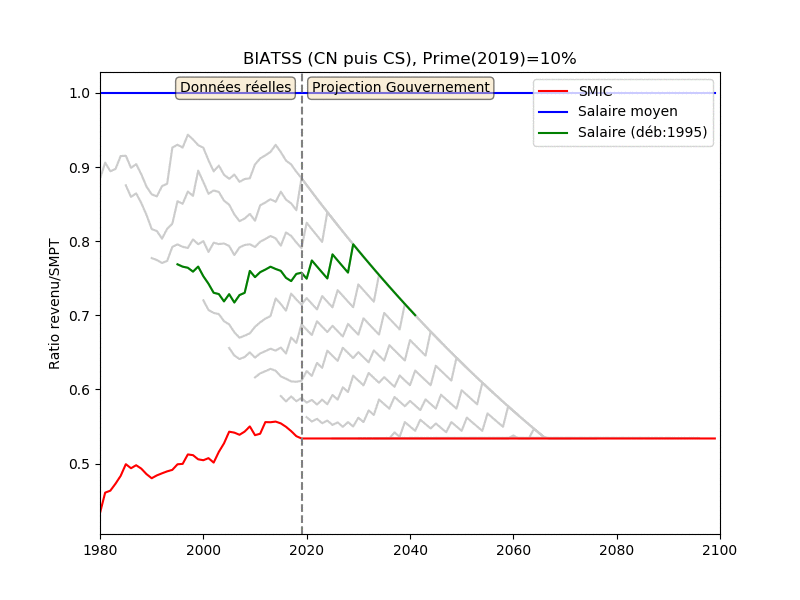
\includegraphics[width=\textwidth]{selonannee-3}}
\frame{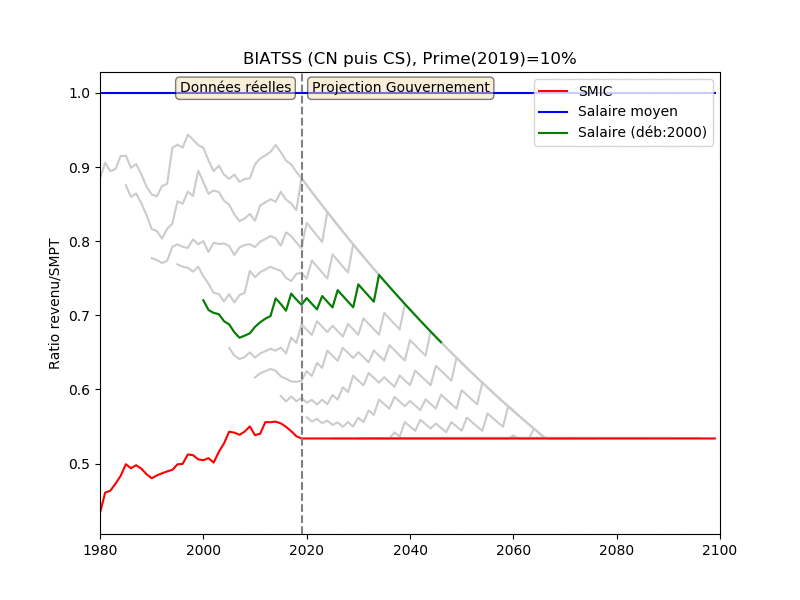
\includegraphics[width=\textwidth]{selonannee-4}}
\frame{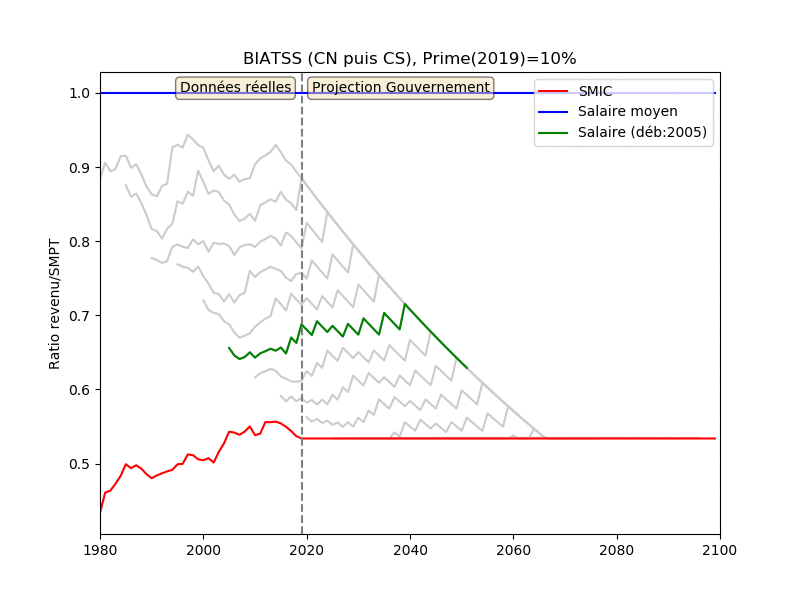
\includegraphics[width=\textwidth]{selonannee-5}}
\frame{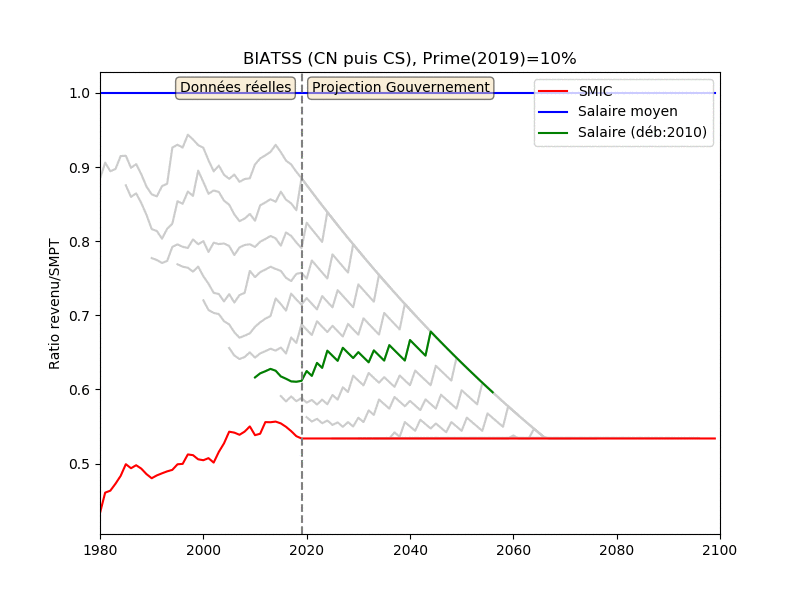
\includegraphics[width=\textwidth]{selonannee-6}}
\frame{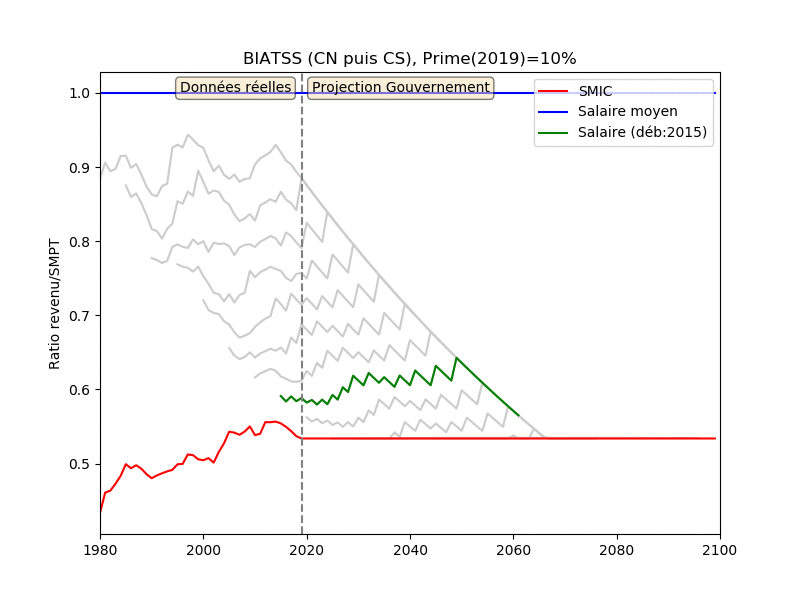
\includegraphics[width=\textwidth]{selonannee-7}}
\frame{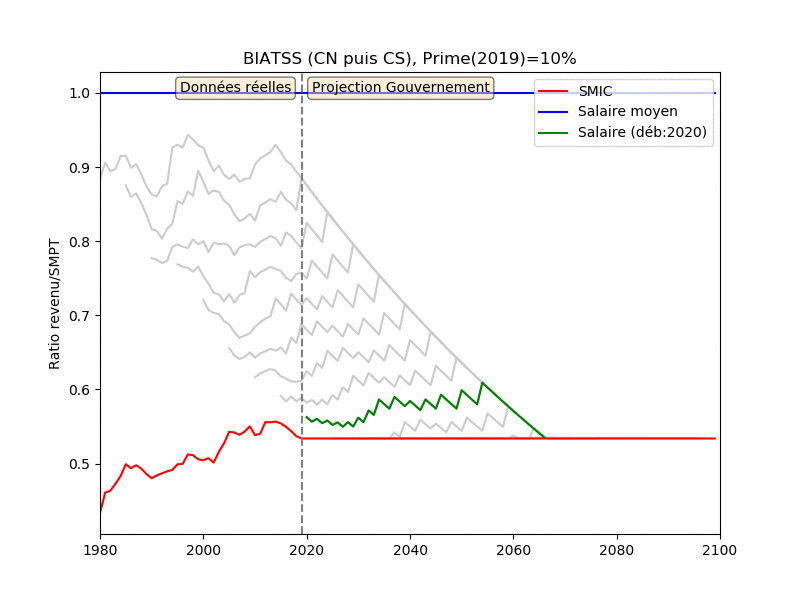
\includegraphics[width=\textwidth]{selonannee-8}}
\frame{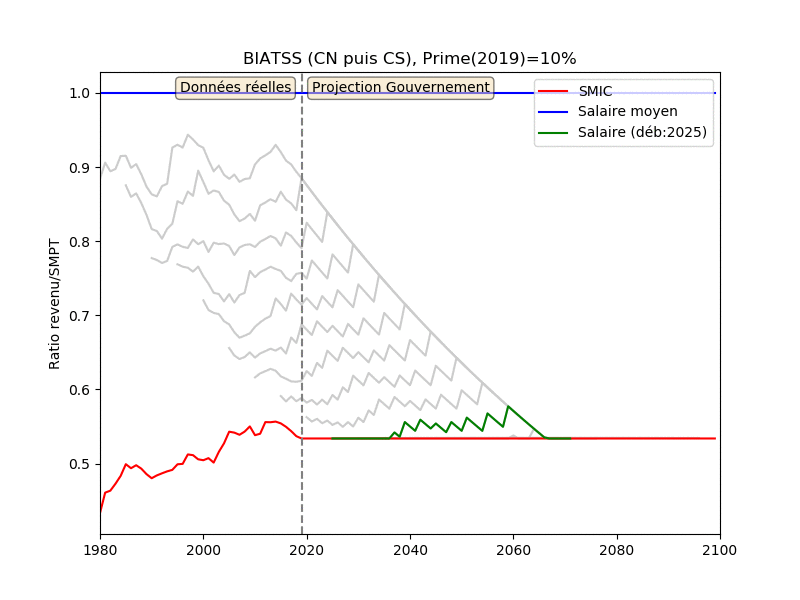
\includegraphics[width=\textwidth]{selonannee-9}}
\frame{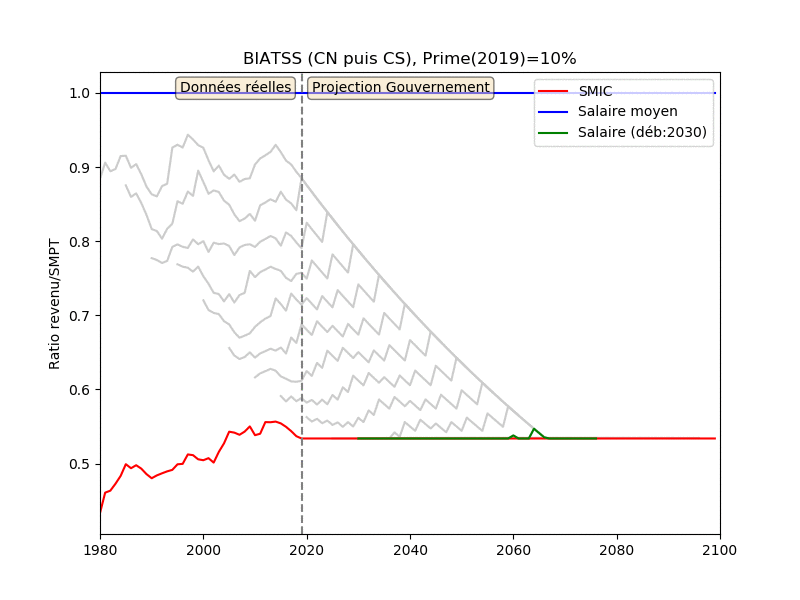
\includegraphics[width=\textwidth]{selonannee-10}}
\frame{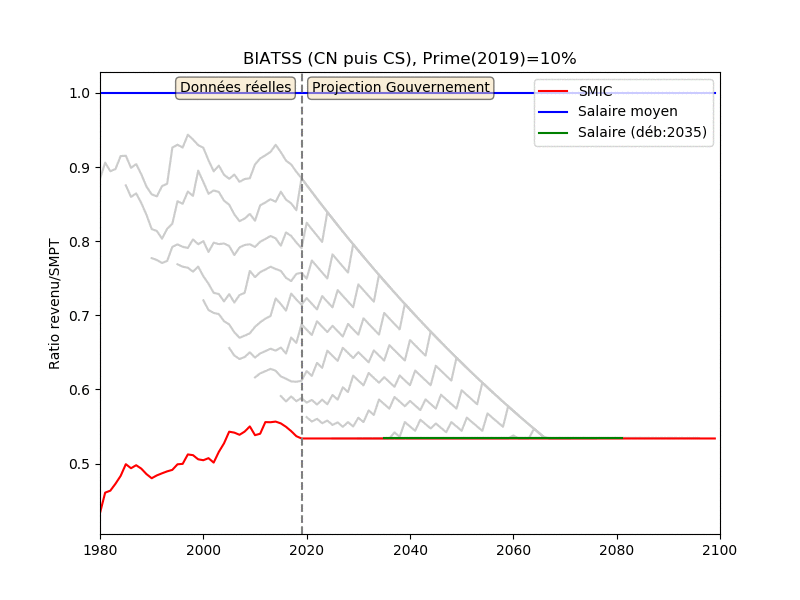
\includegraphics[width=\textwidth]{selonannee-11}}

\frame{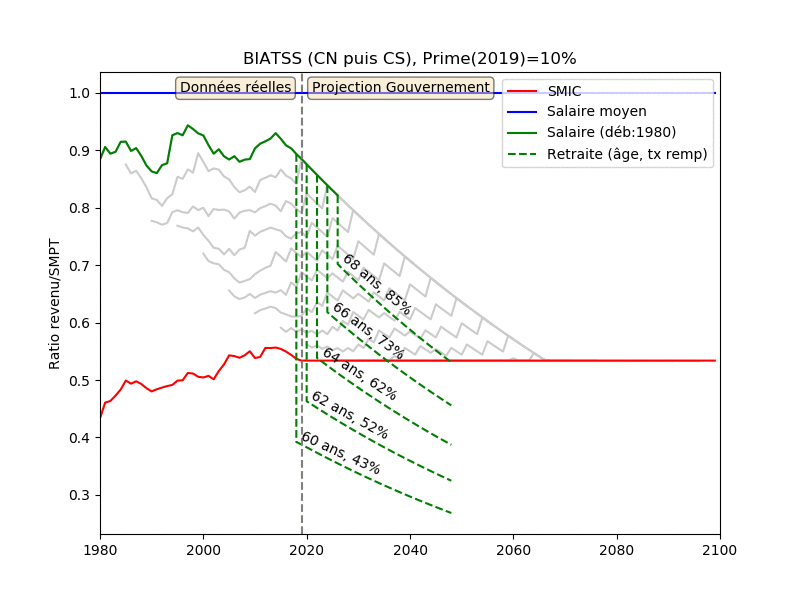
\includegraphics[width=\textwidth]{selonannee_retraite-0}}
\frame{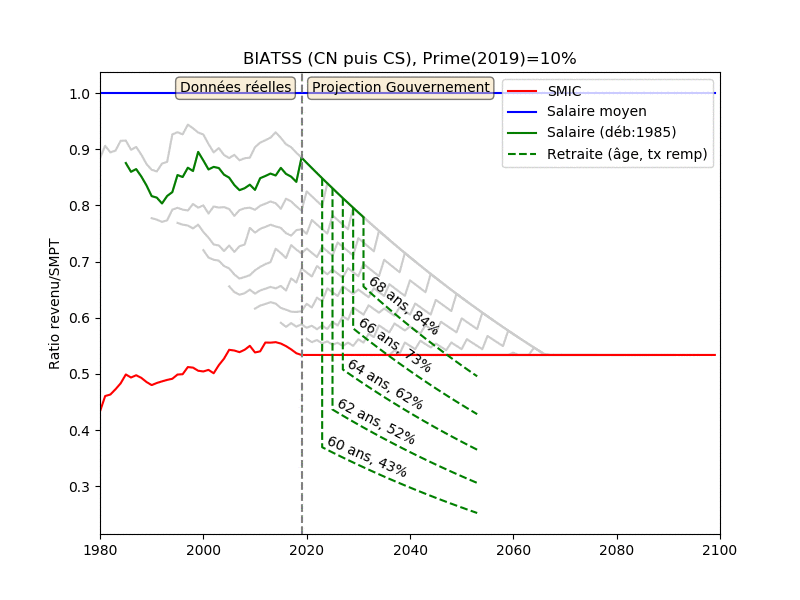
\includegraphics[width=\textwidth]{selonannee_retraite-1}}
\frame{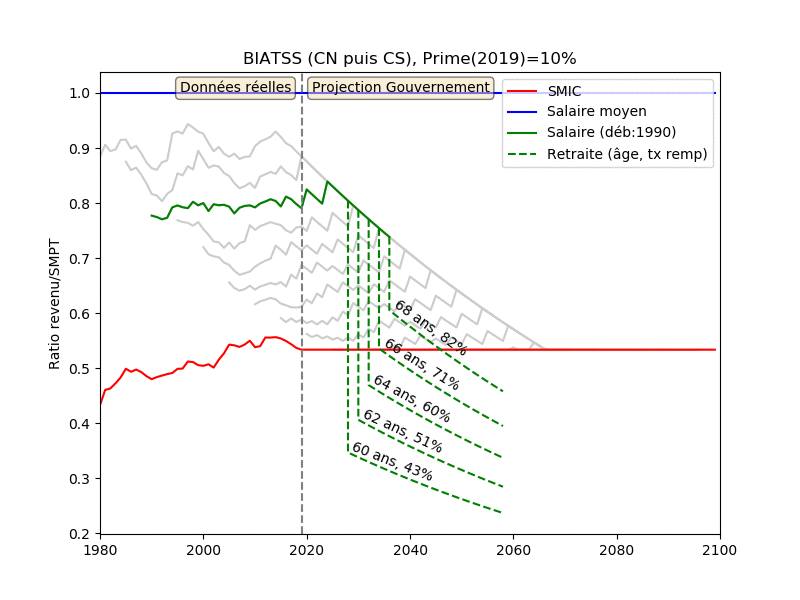
\includegraphics[width=\textwidth]{selonannee_retraite-2}}
\frame{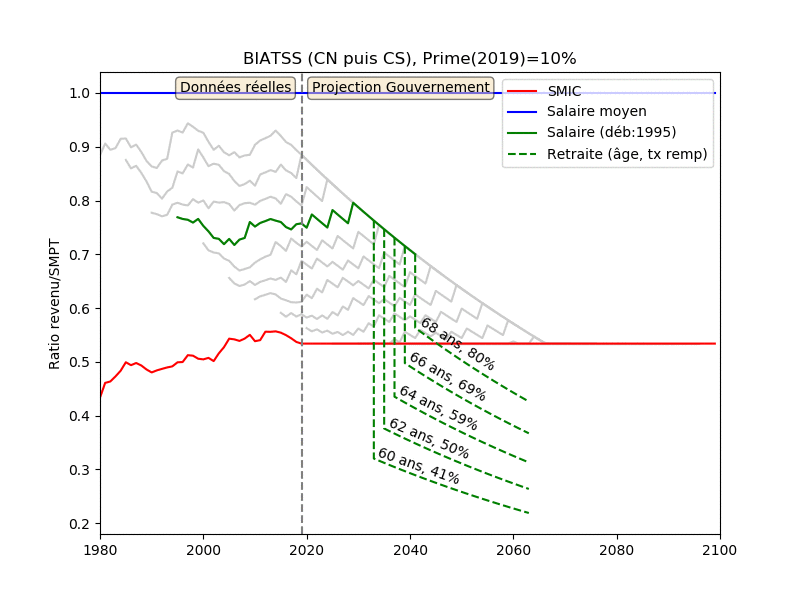
\includegraphics[width=\textwidth]{selonannee_retraite-3}}
\frame{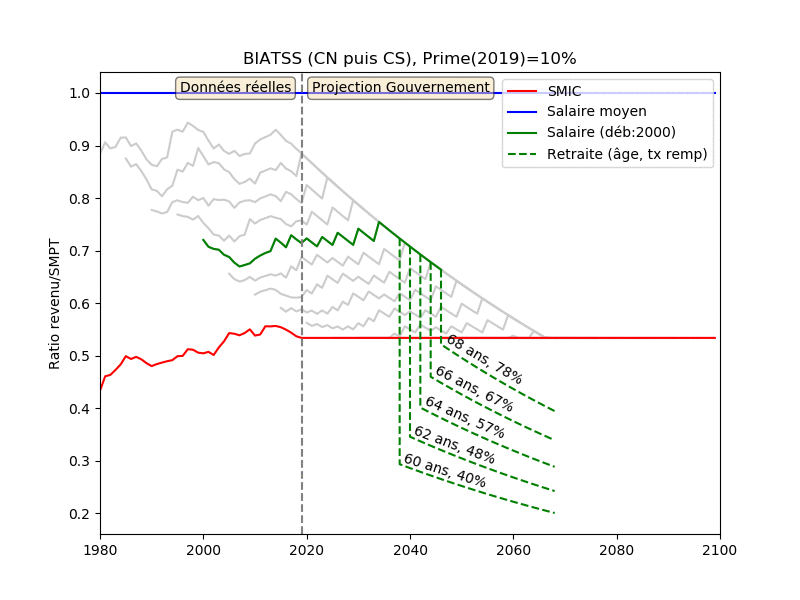
\includegraphics[width=\textwidth]{selonannee_retraite-4}}
\frame{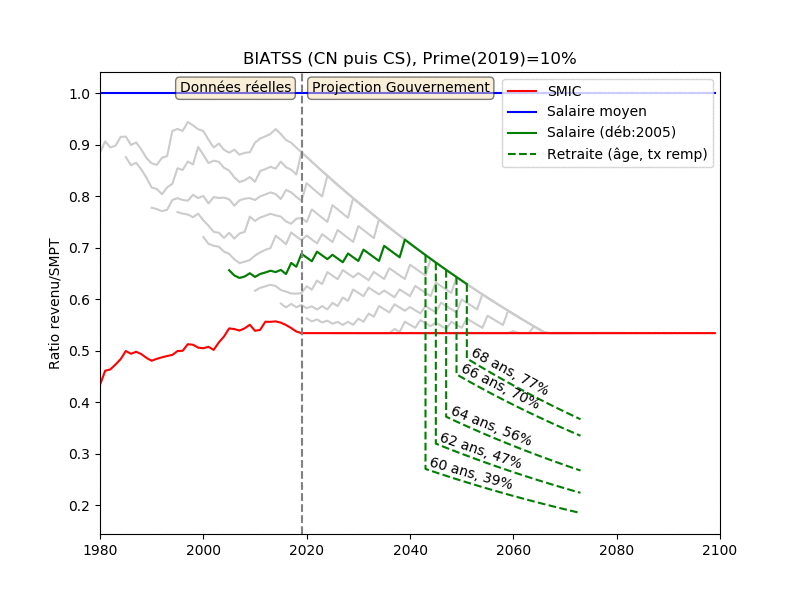
\includegraphics[width=\textwidth]{selonannee_retraite-5}}
\frame{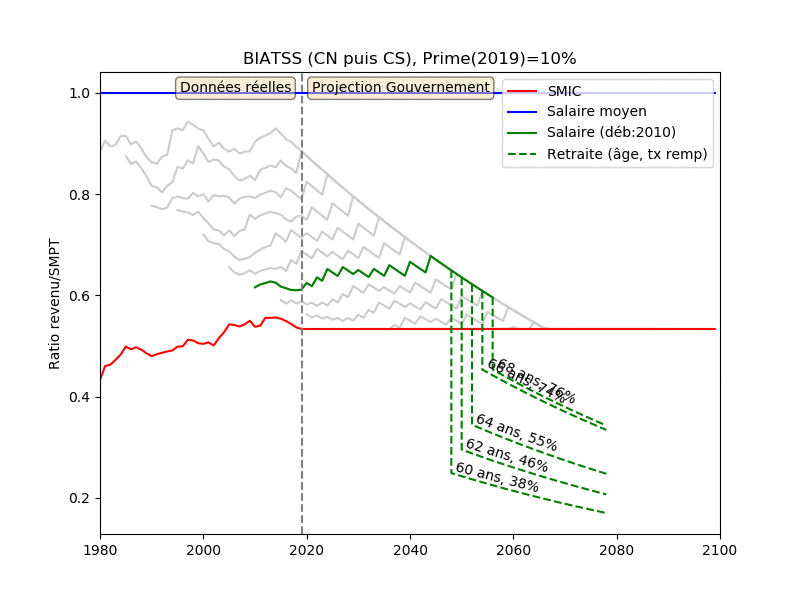
\includegraphics[width=\textwidth]{selonannee_retraite-6}}
\frame{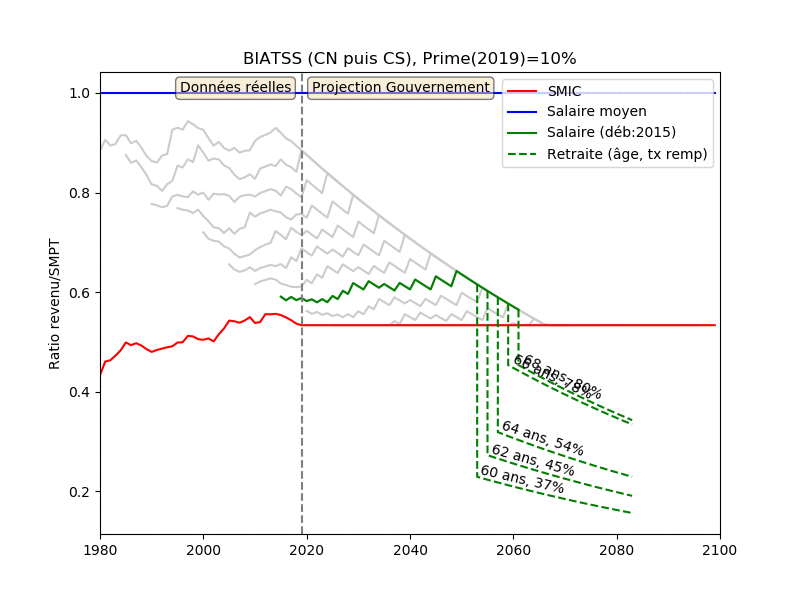
\includegraphics[width=\textwidth]{selonannee_retraite-7}}
\frame{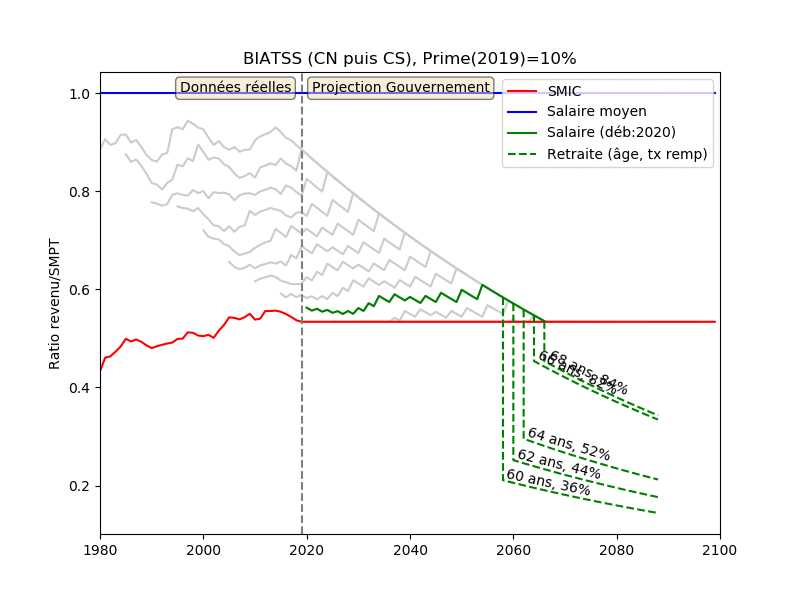
\includegraphics[width=\textwidth]{selonannee_retraite-8}}
\frame{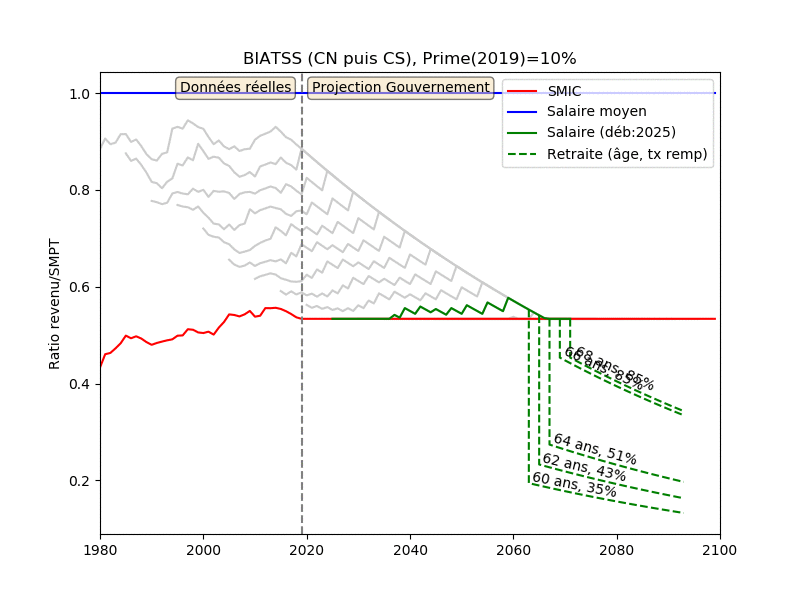
\includegraphics[width=\textwidth]{selonannee_retraite-9}}
\frame{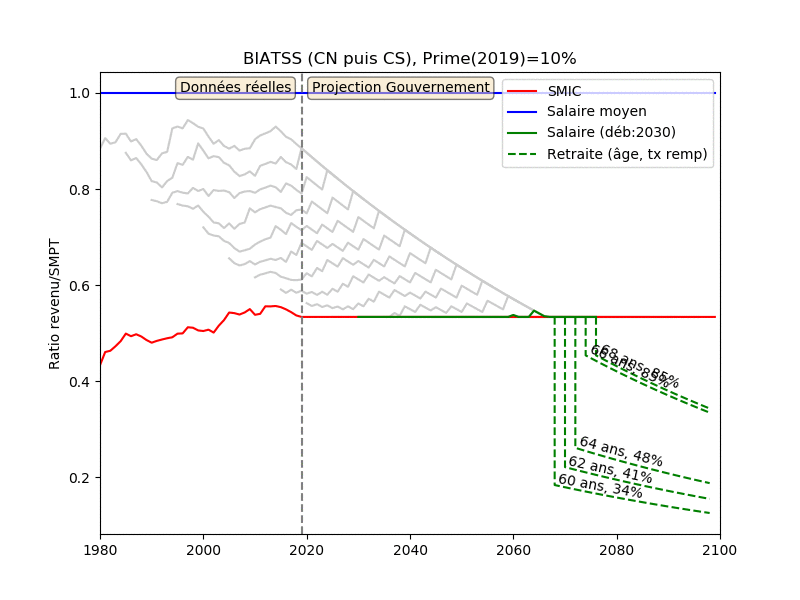
\includegraphics[width=\textwidth]{selonannee_retraite-10}}
\frame{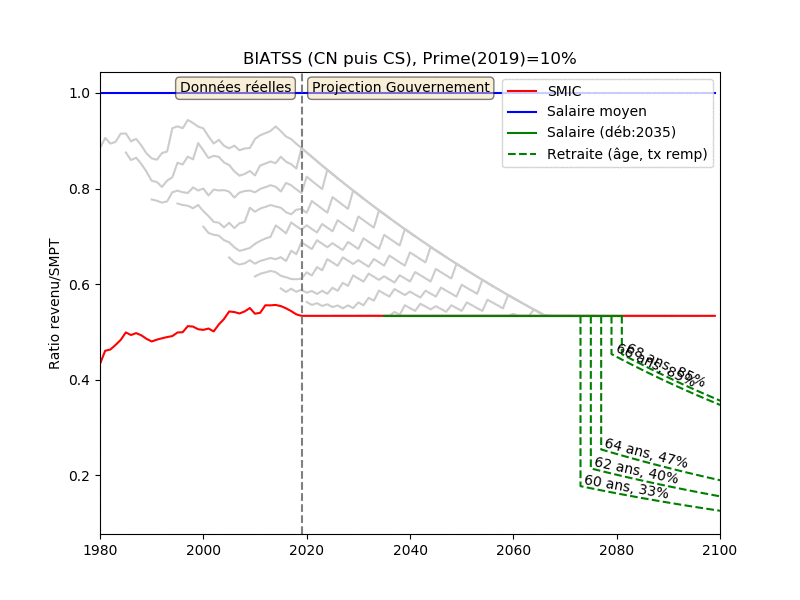
\includegraphics[width=\textwidth]{selonannee_retraite-11}}

\end{document}
